\documentclass[12pt]{report}
\usepackage[utf8]{inputenc}
\usepackage[russian]{babel}
%\usepackage[14pt]{extsizes}
\usepackage{listings}
\usepackage{graphicx}
\usepackage{amsmath,amsfonts,amssymb,amsthm,mathtools} 
\usepackage{pgfplots}
\usepackage{filecontents}
\usepackage{float}
\usepackage{comment}
\usepackage{indentfirst}
\usepackage{caption}
\usepackage{eucal}
\usepackage{enumitem}
%s\documentclass[openany]{book}
\frenchspacing
\setcounter{page}{2} 

\usepackage{indentfirst} % Красная строка

\usetikzlibrary{datavisualization}
\usetikzlibrary{datavisualization.formats.functions}

\usepackage{amsmath}


% Для листинга кода:
\lstset{ %
	language=c,                 % выбор языка для подсветки (здесь это С)
	basicstyle=\small\sffamily, % размер и начертание шрифта для подсветки кода
	numbers=left,               % где поставить нумерацию строк (слева\справа)
	numberstyle=\tiny,           % размер шрифта для номеров строк
	stepnumber=1,                   % размер шага между двумя номерами строк
	numbersep=5pt,                % как далеко отстоят номера строк от подсвечиваемого кода
	showspaces=false,            % показывать или нет пробелы специальными отступами
	showstringspaces=false,      % показывать или нет пробелы в строках
	showtabs=false,             % показывать или нет табуляцию в строках
	frame=single,              % рисовать рамку вокруг кода
	tabsize=2,                 % размер табуляции по умолчанию равен 2 пробелам
	captionpos=t,              % позиция заголовка вверху [t] или внизу [b] 
	breaklines=true,           % автоматически переносить строки (да\нет)
	breakatwhitespace=false, % переносить строки только если есть пробел
	escapeinside={\#*}{*)}   % если нужно добавить комментарии в коде
}


\usepackage[left=2cm,right=2cm, top=2cm,bottom=2cm,bindingoffset=0cm]{geometry}
% Для измененных титулов глав:
\usepackage{titlesec, blindtext, color} % подключаем нужные пакеты
\definecolor{gray75}{gray}{0.75} % определяем цвет
\newcommand{\hsp}{\hspace{20pt}} % длина линии в 20pt
% titleformat определяет стиль
\titleformat{\chapter}[hang]{\Huge\bfseries}{\thechapter\hsp\textcolor{gray75}{|}\hsp}{0pt}{\Huge\bfseries}


% plot
\usepackage{pgfplots}
\usepackage{filecontents}
\usetikzlibrary{datavisualization}
\usetikzlibrary{datavisualization.formats.functions}

\newcommand{\imgw}[3] {
	\begin{figure}[h]
		\centering
		\includegraphics[width=#1]{#2}
		\caption{#3}
		\label{img:#2}
	\end{figure}
}

\begin{document}
	%\def\chaptername{} % убирает "Глава"
	\thispagestyle{empty}
	\begin{titlepage}
		\noindent \begin{minipage}{0.15\textwidth}
			
\includegraphics[width=\linewidth]{img/b_logo}
		\end{minipage}
		\noindent\begin{minipage}{0.9\textwidth}\centering
			\textbf{Министерство науки и высшего образования Российской Федерации}\\
			\textbf{Федеральное государственное бюджетное образовательное учреждение высшего образования}\\
			\textbf{~~~«Московский государственный технический университет имени Н.Э.~Баумана}\\
			\textbf{(национальный исследовательский университет)»}\\
			\textbf{(МГТУ им. Н.Э.~Баумана)}
		\end{minipage}
		
		\noindent\rule{18cm}{3pt}
		\newline\newline
		\noindent ФАКУЛЬТЕТ $\underline{\text{«Информатика и системы управления»}}$ \newline\newline
		\noindent КАФЕДРА $\underline{\text{«Программное обеспечение ЭВМ и информационные технологии»}}$\newline\newline\newline\newline\newline
		
		\begin{center}
			\noindent\begin{minipage}{1.1\textwidth}\centering
				\Large\textbf{Отчет по лабораторной работе №2}\newline
				\textbf{по дисциплине <<Математическая статистика>>}\newline
			\end{minipage}
		\end{center}
		
		\noindent\textbf{Тема} $\underline{\text{Интервальные оценки}}$\newline\newline
		\noindent\textbf{Студент} $\underline{\text{Леонов В.В.}}$\newline\newline
		\noindent\textbf{Группа} $\underline{\text{ИУ7-66Б}}$\newline\newline
		\noindent\textbf{Оценка (баллы)} $\underline{\text{~~~~~~~~~~~~~~~~~}}$\newline\newline
		\noindent\textbf{Преподаватель} $\underline{\text{Власов П.А., Андреева Т.В.}}$\newline\newline\newline
		
		\begin{center}
			\vfill
			Москва~---~\the\year
			~г.
		\end{center}
	\end{titlepage}
	
\chapter*{Постановка задачи}



\section*{Цель работы}

Построение доверительных интервалов для математического ожидания и дисперсии нормальной случайной величины.

\section*{Содержание работы}
\begin{enumerate}
	\item Для выборки объема $n$ из нормальной генеральной совокупности $X$ реализовать в виде программы на ЭВМ:
	\begin{enumerate}
		\item вычисление точечных оценок $\hat\mu(\vec X_n)$ и $S^2(\vec X_n)$ математического ожидания $MX$ и дисперсии $DX$ соответственно;
		\item вычисление нижней и верхней границ $\underline\mu(\vec X_n)$, $\overline\mu(\vec X_n)$ для $\gamma$-доверительного интервала для математического ожидания $MX$;
		\item вычисление нижней и верхней границ $\underline\sigma^2(\vec X_n)$, $\overline\sigma^2(\vec X_n)$ для $\gamma$-доверительного интервала для дисперсии $DX$.
	\end{enumerate}
	\item Вычислить $\hat\mu$ и $S^2$ для выборки из индивидуального варианта.
	\item Для заданного пользователем уровня доверия $\gamma$ (при построении графиков принять $\gamma$ = 0.9) и $N$ – объёма выборки из индивидуального варианта:
	\begin{enumerate}
		\item на координатной плоскости $Oyn$ построить прямую $y = \hat\mu(\vec{x_N})$, также графики функций $y = \hat\mu(\vec x_n)$, $y = \underline\mu(\vec x_n)$ и $y = \overline\mu(\vec x_n)$ как функций объема $n$ выборки, где $n$ изменяется от 1 до $N$;
		\item на другой координатной плоскости $Ozn$ построить прямую $z = S^2(\vec{x_N})$, также графики функций $z = S^2(\vec x_n)$, $z = \underline\sigma^2(\vec x_n)$ и $z = \overline\sigma^2(\vec x_n)$ как функций объема $n$ выборки, где $n$ изменяется от 1 до $N$.
	\end{enumerate}
\end{enumerate}

\textbf{Вариант 9:}

X = (-8.47, -7.45, -7.12, -8.30, -8.15, -6.01, -5.20, -7.38, -6.76, -9.18, -6.00, -8.08, -7.96, -8.34, -6.82, -8.46, -8.07, -7.04, -7.24, -8.16, -8.20, -8.27, -7.79, -7.37, -7.02, -7.13, -6.99, -7.65, -8.18, -6.71, -8.41, -6.71, -7.04, -9.15, -7.74, -10.11, -8.20, -7.07, -7.63, -8.99, -6.62, -6.23, -7.13, -6.41, -7.06, -7.72, -8.44, -8.85, -8.02, -6.98, -6.08, -7.20, -7.48, -7.82, -9.19, -8.31, -7.95, -7.97, -6.66, -6.59, -9.10, -7.87, -9.02, -8.77, -7.62, -9.44, -8.05, -7.60, -7.33, -6.94, -8.51, -7.39, -6.44, -8.88, -8.21, -7.66, -6.91, -8.39, -7.37, -7.26, -6.04, -7.58, -7.28, -7.02, -7.10, -7.33, -8.63, -8.21, -7.12, -8.11, -9.03, -8.11, -8.79, -9.22, -7.32, -5.97, -7.26, -6.39, -7.64, -8.38, -7.67, -7.70, -7.70, -8.95, -6.25, -8.09, -7.85, -8.10, -7.73, -6.78, -7.78, -8.20, -8.88, -8.51, -7.45, -7.14, -6.63, -7.38, -7.72, -6.25)

\clearpage

\chapter*{Общие теоретические сведения}

Дана случайная величина $X$, закон распределения которой известен с точностью до неизвестного параметра $\theta$.

Интервальной оценкой с уровнем доверия $\gamma$ ($\gamma$-доверительной интервальной оценкой) параметра $\theta$ называют пару статистик $\underline{\theta}(\vec X), \overline{\theta}(\vec X)$ таких, что

\begin{equation*}
	P\{\underline{\theta}(\vec X)<\theta<\overline{\theta}(\vec X)\}=\gamma
\end{equation*}

Поскольку границы интервала являются случайными величинами, то для различных реализаций случайной выборки $\vec X$ статистики $\underline{\theta}(\vec X), \overline{\theta}(\vec X)$ могут принимать различные значения.

Доверительным интервалом с уровнем доверия $\gamma$ ($\gamma$-доверительным интервалом) называют интервал $(\underline{\theta}(\vec x), \overline{\theta}(\vec x))$, отвечающий выборочным значениям статистик $\underline{\theta}(\vec X), \overline{\theta}(\vec X)$.

Напишем формулы для вычисления границ $\gamma$-доверительного интервала для 
математического ожидания и дисперсии нормальной случайной величины при условии, что 
их теоретические значения не известны.

Формулы для вычисления границ $\gamma$-доверительного интервала для математического ожидания:

\begin{equation}
	\underline\mu(\vec X_n)=\overline X + \frac{S(\vec X)t^{St(n-1)}_{\frac{1-\gamma}{2}}}{\sqrt{n}}; \overline\mu(\vec X_n)=\overline X + \frac{S(\vec X)t^{St(n-1)}_{\frac{1+\gamma}{2}}}{\sqrt{n}}
\end{equation}


$\overline X$ -- точечная оценка математического ожидания;

$S(\vec X) = \sqrtsign{S^2(\vec X)}$ -- квадратный корень из точечной оценки дисперсии;

$n$ -- объем выборки;

$\gamma$ -- уровень доверия;

$t^{St(n-1)}_{\alpha}$ -- квантиль уровня $\alpha$ распределения Стьюдента с $n - 1$ степенями свободы.

Формулы для вычисления границ $\gamma$-доверительного интервала для дисперсии:

\begin{equation}
	\underline\sigma(\vec X_n)= \frac{(n-1)S^2(\vec X)}{t^{\chi^2(n-1)}_{\frac{1+\gamma}{2}}}; \overline\sigma(\vec X_n)= \frac{(n-1)S^2(\vec X)}{t^{\chi^2(n-1)}_{\frac{1-\gamma}{2}}}
\end{equation}

$S^2(\vec X)$ -- точечная оценка дисперсии;

$n$ -- объем выборки;

$\gamma$ -- уровень доверия;

$t^{\chi^2(n-1)}_{\alpha}$ -- квантиль уровня $\alpha$ распределения $\chi^2$ с $n - 1$ степенями свободы.

\chapter*{Ход работы}
Для решения поставленной задачи была использованна программа \textit{MATLAB 2022a}.

\subsection*{Листинг программы}
\begin{lstlisting}
X = [-8.47, -7.45, -7.12, -8.30, -8.15, -6.01, -5.20, -7.38, -6.76, -9.18, -6.00, -8.08, -7.96, -8.34, -6.82, -8.46, -8.07, -7.04, -7.24, -8.16, -8.20, -8.27, -7.79, -7.37, -7.02, -7.13, -6.99, -7.65, -8.18, -6.71, -8.41, -6.71, -7.04, -9.15, -7.74, -10.11, -8.20, -7.07, -7.63, -8.99, -6.62, -6.23, -7.13, -6.41, -7.06, -7.72, -8.44, -8.85, -8.02, -6.98, -6.08, -7.20, -7.48, -7.82, -9.19, -8.31, -7.95, -7.97, -6.66, -6.59, -9.10, -7.87, -9.02, -8.77, -7.62, -9.44, -8.05, -7.60, -7.33, -6.94, -8.51, -7.39, -6.44, -8.88, -8.21, -7.66, -6.91, -8.39, -7.37, -7.26, -6.04, -7.58, -7.28, -7.02, -7.10, -7.33, -8.63, -8.21, -7.12, -8.11, -9.03, -8.11, -8.79, -9.22, -7.32, -5.97, -7.26, -6.39, -7.64, -8.38, -7.67, -7.70, -7.70, -8.95, -6.25, -8.09, -7.85, -8.10, -7.73, -6.78, -7.78, -8.20, -8.88, -8.51, -7.45, -7.14, -6.63, -7.38, -7.72, -6.25];
gamma = 0.9;

% 1-2
[muhat, muci] = my_normfit_mu(X, 1 - gamma);
[s2hat, s2ci] = my_normfit_s2(X, 1 - gamma);
fprintf("mu = %f\nmu_bottom = %f\nmu_top = %f\n", muhat, muci(1), muci(2));
fprintf("s2 = %f\ns2_bottom = %f\ns2_top = %f\n", s2hat, s2ci(1), s2ci(2));
% 3
process_mu(X, gamma, muhat);
process_s2(X, gamma, s2hat);


function [muhat, muci] = normfit_mu(X, alpha)
	[muhat, ~, muci, ~] = normfit(X, alpha);
end

function [s2hat, s2ci] = normfit_s2(X, alpha)
	[~, sigmahat, ~, sigmaci] = normfit(X, alpha);
	s2hat = sigmahat ^ 2;
	s2ci = sigmaci .^ 2;
end


function [muhat, muci] = my_normfit_mu(X, alpha)
	muhat = mean(X);
	s = std(X);
	gamma = 1 - alpha;
	n = length(X);
	mu_bottom = muhat + s * tinv((1 - gamma) / 2, n - 1) / sqrt(n);
	mu_top = muhat + s * tinv((1 + gamma) / 2, n - 1) / sqrt(n);
	muci = [mu_bottom, mu_top];
end

function [s2hat, s2ci] = my_normfit_s2(X, alpha)
	s2hat = var(X);
	gamma = 1 - alpha;
	n = length(X);
	s2_top = (n - 1) * s2hat / chi2inv((1 - gamma) / 2, n - 1);
	s2_bottom = (n - 1) * s2hat / chi2inv((1 + gamma) / 2, n - 1);
	s2ci = [s2_bottom, s2_top];
end

function process_parameter(start, X, gamma, est, fit, line_legend, est_legend, top_legend, bottom_legend)
	N = length(X);
	figure;
	hold on;
	grid on;
	plot([1, N], [est, est]);
	ests = [];
	cis_bottom = [];
	cis_top = [];
	for n = start:N
		[est, cis] = fit(X(1:n), 1 - gamma);
		ests = [ests, est];
		cis_bottom = [cis_bottom, cis(1)];
		cis_top = [cis_top, cis(2)];
	end
	plot(start:N, ests);
	plot(start:N, cis_bottom);
	plot(start:N, cis_top);
	l = legend(line_legend, est_legend, top_legend, bottom_legend);
	set(l, 'Interpreter', 'latex', 'fontsize', 18);
	hold off;
end

function process_mu(X, gamma, muhat)
	process_parameter(1, X, gamma, muhat, @my_normfit_mu, '$\hat\mu(\vec x_N)$', '$\hat\mu(\vec x_n)$', '$\underline\mu(\vec x_n)$', '$\overline\mu(\vec x_n)$');
end


function process_s2(X, gamma, S2)
	process_parameter(10, X, gamma, S2, @my_normfit_s2, '$\hat\sigma^2(\vec x_N)$', '$\hat\sigma^2(\vec x_n)$', '$\underline\sigma^2(\vec x_n)$', '$\overline\sigma^2(\vec x_n)$');
end
\end{lstlisting}

\subsection*{Результат работы программы}

\begin{table}[h!]
	\centering
\begin{tabular}{l|l|l|l|l|l|l} 
	& $\hat\mu(\vec x_n)$  & $S^2(\vec x_n)$  & $\underline\mu(\vec x_n)$ & $\overline\mu(\vec x_n)$ & $\underline{S^2}(\vec x_n)$  & $\overline{S^2}(\vec x_n)$ \\ \hline
	$\gamma = 0.95$& $-7.660917$  & $0.777892$  & $-7.820342$  & $-7.501492$  & $0.612699$ & $1.020613$ \\ \hline
	$\gamma = 0.9$& $-7.660917$  & $0.777892$ & $-7.794389$ & $-7.527445$ & $0.636386$  & $0.976353$  \\ \hline
	$\gamma = 0.8$& $-7.660917$  & $0.777892$  & $-7.764675$  & $-7.557158$  & $0.665250$  & $0.928415$ \\ 
\end{tabular}	
\end{table}

	Таким образом, при увелечении/уменьшении уровня доверия $\gamma$ доверительный интервал увеличивается/уменьшается соответственно.

\newpage

\captionsetup{justification=centering}

\begin{figure}[h!]
	\centering
	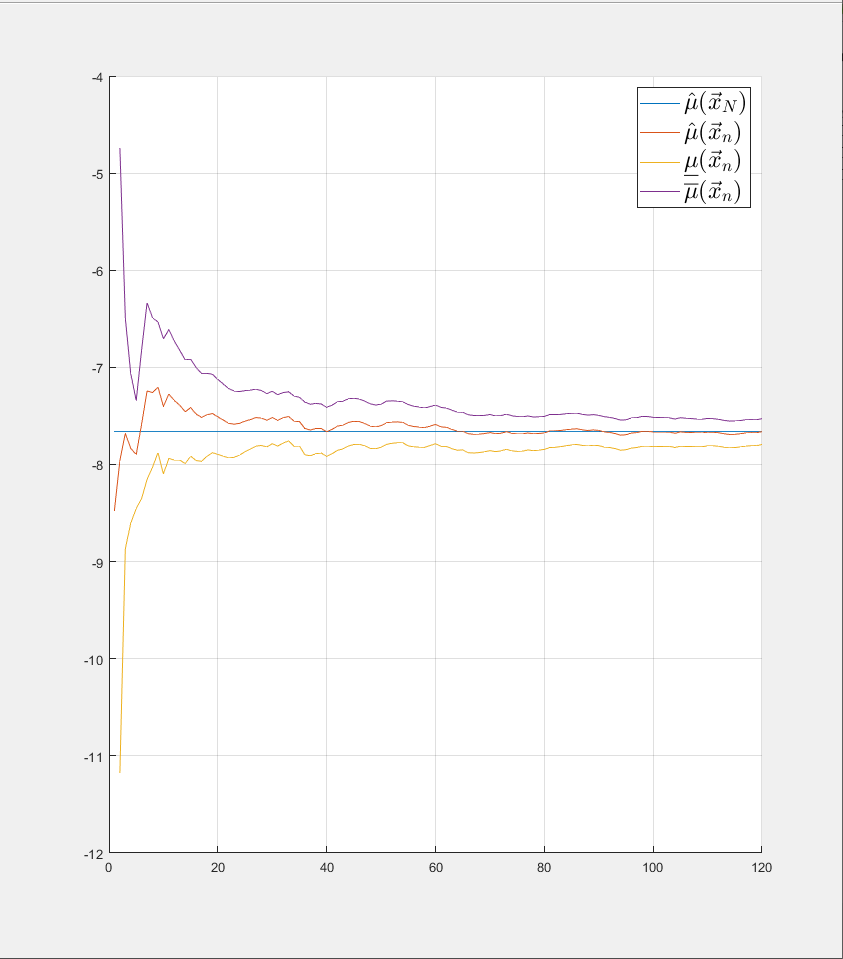
\includegraphics[width=\textwidth]{img/f1}
	\caption{Прямая $y(n) = \hat\mu(\vec x_N)$, а также графики функций $y(n) = \underline\mu(\vec x_n)$, $y(n) = \overline\mu(\vec x_n)$, $y(n) = \hat\mu(\vec x_n)$ как функций объема $n$ выборки, где $n$ изменяется от 1 до $N$}
\end{figure}

\newpage

\begin{figure}[h!]
	\centering
	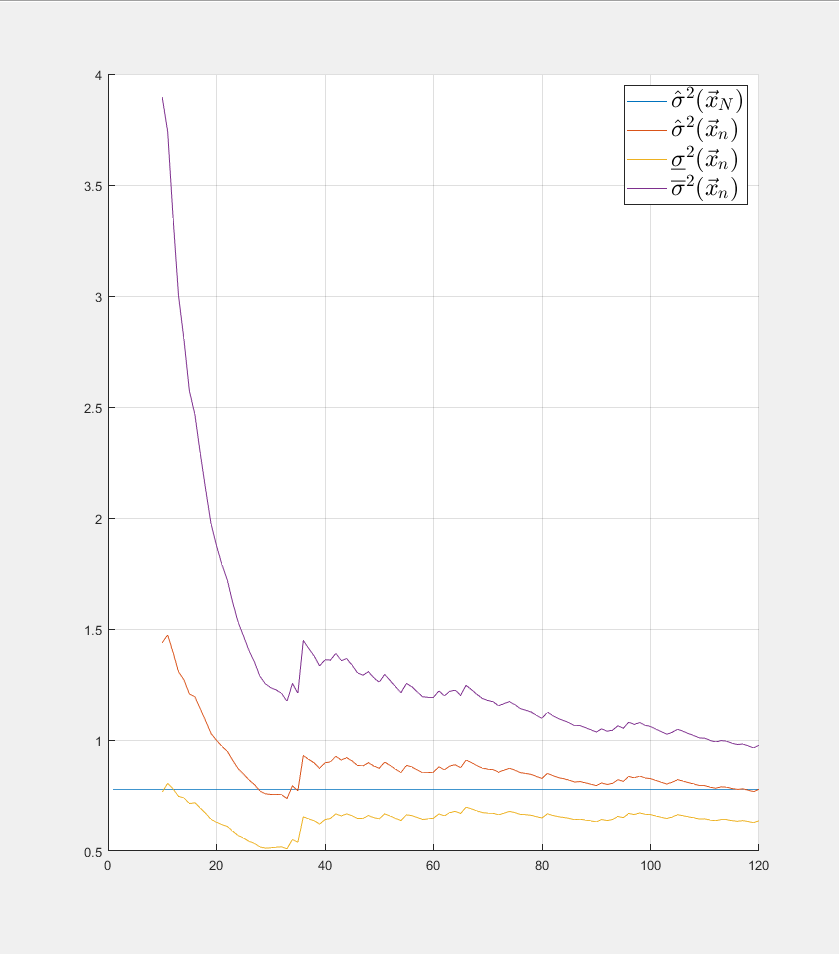
\includegraphics[width=\textwidth]{img/f2}
	\caption{Прямая $z(n) = \hat S^2(\vec x_N)$, а также графики функций $z(n) = \underline S^2(\vec x_n)$, $z(n) = \overline S^2(\vec x_n)$, $z(n) = \hat S^2(\vec x_n)$ как функций объема $n$ выборки, где $n$ изменяется от 10 до $N$}
\end{figure}

\bibliographystyle{utf8gost705u}  % стилевой файл для оформления по ГОСТу
\bibliography{51-biblio}          % имя библиографической базы (bib-файла)
	
\end{document}
